\documentclass[a4paper,10pt]{article}
\usepackage[utf8]{inputenc}
\usepackage{amsmath}
\usepackage{caption}
\usepackage{graphicx}
\usepackage{enumerate}
\usepackage{cite}
\title{Lazy Caterer's Sequence}
\author{William Peters, Gihan Mendis}

\begin{document}

\maketitle

\section{Illustration of structures}

\subsection{Pancake Structure}
\begin{enumerate}
  \item $n = 4$\\
  	\begin{enumerate}
    	\item Pancake structure\\
    	\begin{figure}[h!]
			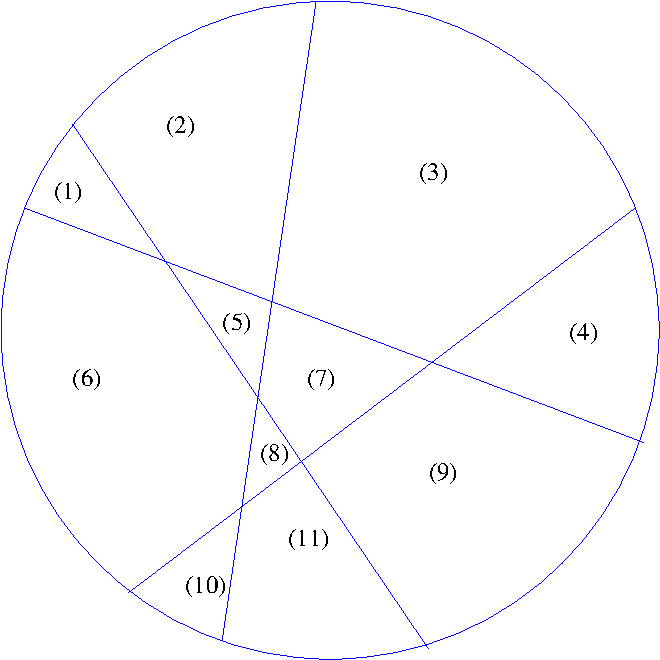
\includegraphics[scale=0.3]{graphics/pancakecut11}
			\captionsetup{labelformat=empty}
			\caption{}
			\label{fig:pancakecut11}
		\end{figure}
  \end{enumerate}
  
  %This should be n = 5 not 4 
  \item $n = 5$\\
  \begin{enumerate}
    \item Pancake structure\\
      \begin{figure}[h!]
			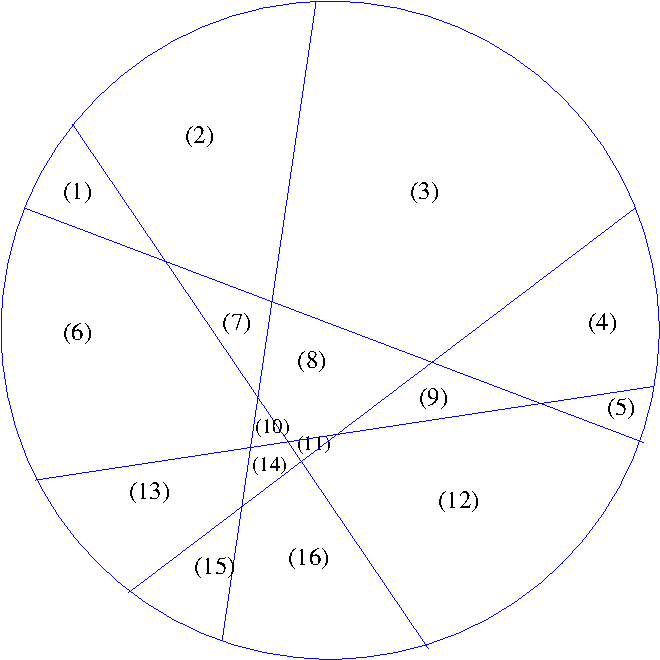
\includegraphics[scale=0.3]{graphics/pancakecut16}
			\captionsetup{labelformat=empty}
			\caption{}
			\label{fig:pancakecut16}
		\end{figure}
  \end{enumerate}
\end{enumerate}

\subsection{Binary Words}
When $n > 3$  the sequence gives the number of binary words where there are at least two ones and at most two two's. In these formulas $n$ represents the length of a binary word, so $a(n)$ gives the number of possible binary words formed with these constraints. The following are two illustrations of this structure. The first is when $n = 4$ and the second is when $n = 5$.

\begin{enumerate}
	\item $n = 4$\\
	\begin{enumerate}
		\item Binary words structure illustration\\
		\[
		\boxed{
		\begin{gathered}
		0011, 0101, 0110, 0111, 1001, 1010, 1011, 1100, 1101, 1110, 1111
		\end{gathered}
		}
		\]
	\end{enumerate}
	
	\item $n = 5$\\
	\begin{enumerate}
		\item Binary words structure illustration\\
		\[
		\boxed{
		\begin{gathered}
		11111, 01111, 10111, 11011, 11101, 11110, 00111, 10011, 10101, 10110,\\ 		        01011, 01101, 01110, 11100, 11001, 11010 
		\end{gathered}
		}
		\]
	\end{enumerate}
\end{enumerate}
 
\section{Formula Demonstrations}
\subsection{Binomial}
\begin{enumerate}
 \item $a(n) = Binomial(n+2,1)-2\times Binomial(n+1,1)+Binomial(n+2,2)$\\

  \hspace{1cm}${n+2 \choose 1} - 2\times {n+1 \choose 1} + {n+2 \choose 2}$\\
  \begin{enumerate}
    \item $n = 4$
    \[
     \boxed{ 
	  \begin{gathered}
       	a(4) = {4+2 \choose 1} - 2\times {4+1 \choose 1} + {4+2 \choose 2}\\
		\\ 
       	a(4) = {6 \choose 1} - 2\times {5 \choose 1} + {6 \choose 2} \\
       	\\
       	a(4) = 6 - 10 + 15\\
       	\\
       	a(4) = 11 
      \end{gathered}	    
	  }
    \]	  
    \item $ n = 5$
    \[
     \boxed{ 
	  \begin{gathered}
       	a(5) = {5+2 \choose 1} - 2\times {5+1 \choose 1} + {5+2 \choose 2}\\
		\\ 
       	a(5) = {7 \choose 1} - 2\times {6 \choose 1} + {7 \choose 2} \\
       	\\
       	a(5) = 7 - 12 + 21\\
       	\\
       	a(4) = 16 
      \end{gathered}	    
	  }
    \]	
  \end{enumerate}
\end{enumerate}

\subsection{Generating Function}
\begin{enumerate}
\item $G.f : A(x) = (1-x+x^2)/(1-x)^3$
  \begin{enumerate}
    \item $n = 4$
    \[
     \boxed{ 
	  \begin{gathered}
    	{[}\frac{d^4 }{dx^4}(1-x+x^2)/(1-x)^3 {]}_{x=0} = 264  \\ 
    	And ~ \frac{264}{4!} = 11 \\
      \end{gathered}	    
	  }
    \]	  
    \item $ n = 5$
    \[
     \boxed{ 
	  \begin{gathered}
		{[}\frac{d^5 }{dx^5}(1-x+x^2)/(1-x)^3 {]}_{x=0} = 1920  \\ 
    	And ~ \frac{1920}{5!} = 16 \\
      \end{gathered}	    
	  }
    \]	
  \end{enumerate}
\end{enumerate}

\subsection{Exponential Generating Function}
\begin{enumerate}
\item $E.g.f: A(x) = e^x+xe^x+\frac{e^xx^2}{2}$
	\begin{enumerate}
		\item $n = 4$
		\[
		\boxed{
			\begin{gathered}
				{[}\frac{d^4}{dx^4}(e^x+xe^x+\frac{e^xx^2}{2}){]}_{x=0} = 11
			\end{gathered}
		}
		\]
		\item $ n = 5$
		\[
		\boxed{
			\begin{gathered}
				{[}\frac{d^5}{dx^5}(e^x+xe^x+\frac{e^xx^2}{2}){]}_{x=0} = 16
			\end{gathered}
		}
		\]
	\end{enumerate}
\end{enumerate}

\subsection{Recursive Formula}
\begin{enumerate}
\item $ a(n+3) = 3*a(n+2)-3*a(n+1) + a(n), a(0) = 1, a(1) = 2, a(2) = 4, a(3) = 7, a(4) = 11, a(5) = 16, a(6) = 22, a(7) = 29, a(8) = 37 $
	\begin{enumerate}
		\item $n = 6$
		\[
		\boxed{
			\begin{gathered}
				a(6+3) = a(9) = 3*a(6+2) - 3*a(6+1) + a(6)\\
				\\
				a(9) = 3*a(8) - 3*a(7) + a(6)\\
				\\
				a(9) = 3*37 - 3*29 + 22\\
				\\
				a(9) = 111-87+22 = 46
			\end{gathered}
			}
		\]
		
		\item $n = 7$
		\[
		\boxed{
			\begin{gathered}
				a(7+3) = a(10) = 3*a(7+2) - 3*a(7+1) + a(7)\\
				\\
				a(10) = 3*a(10) - 3*a(8) + a(7)\\
				\\
				a(10) = 3*46 - 3*37 + 29\\
				\\
				a(10) = 138-111+29 = 56
			\end{gathered}
			}
		\]
		
		\item $n = 8$
		\[
		\boxed{
			\begin{gathered}
				a(8+3) = a(11) = 3*a(8+2) - 3*a(8+1) + a(8)\\
				\\
				a(11) = 3*a(10) - 3*a(9) + a(8)\\
				\\
				a(11) = 3*56 - 3*46 + 37\\
				\\
				a(11) = 168-138+37 = 67
			\end{gathered}
			}
		\]
	\end{enumerate}

\end{enumerate}

\section{Experimental Bijection}

We attempt to define a rule that map maximum set of pancake pieces we can get from n cuts to set of $n$ wordlenght binary words where there are at least two ones and at most two two's. (When  $n > 3$) : \\
\\
We label each pancake cut from "1" to "n" and the original boundary of pancake as "0". Then we consider the boundaries of each piece in alphabetize order as an unique representation of each piece. We attempt to find the bijection of this representation of pancake structure to other binary word structure.\\
\\
Our attempt was illustrated below for when $n=4$.    	    
\\	
\subsection{Demonstration when $n=4$.}
\begin{figure}[h!]
			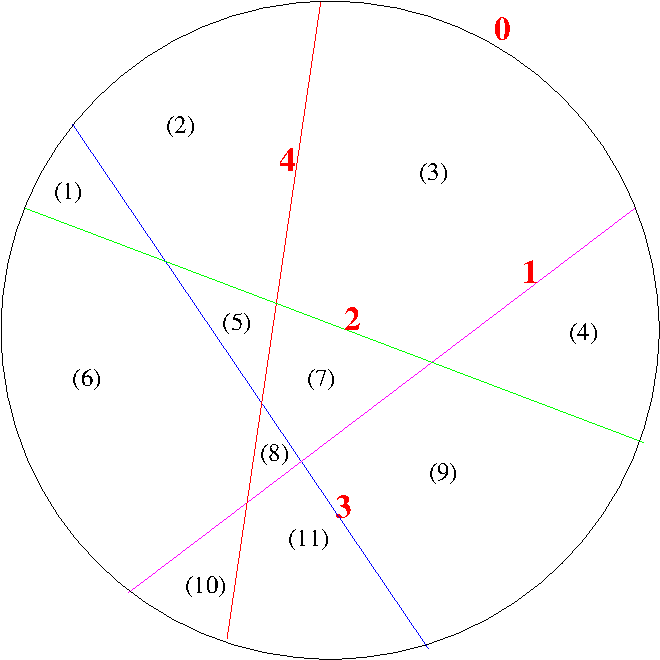
\includegraphics[scale=0.5]{graphics/pancakecut11_bijec}
			\captionsetup{labelformat=empty}
			\caption{}
			\label{fig:pancakecut11}
\end{figure}

By labeling the maximum set of pieces with there boundaries and alphabetize ordering we get the set as follows:\\
\\
${012,0123,01234,0124,0134,014,023,0234,1234,134,234}$ \\
\\
Ordered set of binary number structure is as follows:\\
\\
${0011, 0101, 0110, 0111, 1001, 1010, 1011, 1100, 1101, 1110, 1111}$\\
\\
The bijection we can observe is in the shifting of high digits to the left as we move right. Notice with the alphabetical ordering of the numbers the high values appear to shift left as we move to the right of the ordering. All high values are focused left. There could exist an in depth pattern mapping the shift of these high values to the left as we move right along the ordering. We can notice the circular boundaries right most require a higher number of collection of lines to form the boundaries. Similarly the right most binary words contain a collection of the highest individual bits. We open a question of whether there is a established mapping that can map this phenomena. The question can be seen as a question in partition theory.  

\subsection{Demonstration when $n=5$.}
The same bijection rule and open question holds for when $n=5$\\
\\
The following is the maximum set of pieces with there boundaries alphabetized when $n = 5$\\
\\
${012,0123,0124,01345,0145,0234,02345,025,034,045,12345,1235,135,145,234,235}$\\
\\
Here are the binary words ordered alphabetized when $n=5$\\
\\
${00111, 01011, 01101, 01110, 01111, 10011, 10101, 10110, 10111, 11001, 11010, 11011, 11100, 11101, 11110, 11111}$\\
\\
Notice  how the same pattern holds, our highs tend to shift left most as the ordering moves right.
\section{Experimental Superstructure}

As mentioned in the experimental bijection section the set from the pancake structure can be organize labeling each piece with there boundaries and alphabetize ordering them. The same goes for binary words, we organize them by alphabetizing. Then the superstructure for $n=4$ and $n=5$ are given as bellow. 

\begin{enumerate}
		\item $n=4$\\
		\[
		\boxed{
		\begin{gathered}
	{012,0123,01234,0124,0134,014,023,0234,1234,134,234} \\
	\\
	{0011, 0101, 0110, 0111, 1001, 1010, 1011, 1100, 1101, 1110, 1111}
		\end{gathered}
		}
		\]
		\item $n=5$\\
		\[
		\boxed{
		\begin{gathered}
		{012,0123,0124,01345,0145,0234,02345,025,034,045,12345,1235,135,145,234,235}\\
		\\
		{00111, 01011, 01101, 01110, 01111, 10011, 10101, 10110, 10111, 11001, 11010, 11011, 11100, 11101, 11110, 11111}\\ 
		\end{gathered}
		}
		\]
\end{enumerate}

\section{Open Question}
The Lazy Caterer's Sequence is a very well known sequence. It gives the maximum number of partitions by N lines of a two dimensional plane. Along our research of this sequence we have discovered our own open question about this sequence in general.
\\
The Lazy caterers sequences demonstrates the maximum number of partitions of a circle of plane by $n$ lines in two dimensions. Similarly, there is a sequence that demonstrates this in three dimensions known as the cake numbers.\\
\\
The follow is the first 7 values of the cake numbers, note similarly the sequence begins at $n=0$.\\
\\
$1, 2, 4, 8, 15, 26, 42, 64, 93, 130$\\
\\
One interesting property to notice about this sequence is the subtraction of two sequential values gives a value in the Lazy Caterer's Sequence\\
\\
\[
\boxed{
	\begin{gathered}
		{2-1 = 1}\\
		{4-2 = 2} \\
		{8-4 = 4} \\
		{15-8 = 7} \\
		{26-15 = 11}\\
		{42-26 = 16}\\
		{64-42 = 22}\\
		{93-64 = 29}\\
		{130-93 = 37}\\
	\end{gathered}
	}
\]
\\
This can be seen as a reduction from three dimensional space down into two dimensional space. The question is, does there exist a rule such that we can derive the cake numbers from numbers in the Lazy Caterer's Sequence? This would require a upward shift from two dimensional space into three dimensional space.

\begin{thebibliography}{1}
\bibitem{OEIS}
Online Encyclopedia of Integer Sequences, \\
\texttt{https://oeis.org/A000124}

\bibitem{OEIS}
Online Encyclopedia of Integer Sequences, \\
\texttt{https://oeis.org/A000125}

\end{thebibliography}

\end{document}
